
\let\negmedspace\undefined
\let\negthickspace\undefined
\documentclass[journal,12pt,twocolumn]{IEEEtran}
\usepackage{cite}
\usepackage{amsmath,amssymb,amsfonts,amsthm}
\usepackage{algorithmic}
\usepackage{graphicx}
\usepackage{textcomp}
\usepackage{xcolor}
\usepackage{txfonts}
\usepackage{listings}
\usepackage{enumitem}
\usepackage{mathtools}
\usepackage{gensymb}
\usepackage[breaklinks=true]{hyperref}
\usepackage{tkz-euclide} % loads  TikZ and tkz-base
\usepackage{listings}

\DeclareMathOperator*{\Res}{Res}
%\renewcommand{\baselinestretch}{2}
\renewcommand\thesection{\arabic{section}}
\renewcommand\thesubsection{\thesection.\arabic{subsection}}
\renewcommand\thesubsubsection{\thesubsection.\arabic{subsubsection}}

\renewcommand\thesectiondis{\arabic{section}}
\renewcommand\thesubsectiondis{\thesectiondis.\arabic{subsection}}
\renewcommand\thesubsubsectiondis{\thesubsectiondis.\arabic{subsubsection}}

% correct bad hyphenation here
\hyphenation{op-tical net-works semi-conduc-tor}
\def\inputGnumericTable{}                                 %%

\lstset{
%language=C,
frame=single, 
breaklines=true,
columns=fullflexible
}
%\lstset{
%language=tex,
%frame=single, 
%breaklines=true
%}

\begin{document}
%


\newtheorem{theorem}{Theorem}[section]
\newtheorem{problem}{Problem}
\newtheorem{proposition}{Proposition}[section]
\newtheorem{lemma}{Lemma}[section]
\newtheorem{corollary}[theorem]{Corollary}
\newtheorem{example}{Example}[section]
\newtheorem{definition}[problem]{Definition}
%\newtheorem{thm}{Theorem}[section] 
%\newtheorem{defn}[thm]{Definition}
%\newtheorem{algorithm}{Algorithm}[section]
%\newtheorem{cor}{Corollary}
\newcommand{\BEQA}{\begin{eqnarray}}
\newcommand{\EEQA}{\end{eqnarray}}
\newcommand{\define}{\stackrel{\triangle}{=}}

\bibliographystyle{IEEEtran}
%\bibliographystyle{ieeetr}


\providecommand{\mbf}{\mathbf}
\providecommand{\pr}[1]{\ensuremath{\Pr\left(#1\right)}}
\providecommand{\qfunc}[1]{\ensuremath{Q\left(#1\right)}}
\providecommand{\sbrak}[1]{\ensuremath{{}\left[#1\right]}}
\providecommand{\lsbrak}[1]{\ensuremath{{}\left[#1\right.}}
\providecommand{\rsbrak}[1]{\ensuremath{{}\left.#1\right]}}
\providecommand{\brak}[1]{\ensuremath{\left(#1\right)}}
\providecommand{\lbrak}[1]{\ensuremath{\left(#1\right.}}
\providecommand{\rbrak}[1]{\ensuremath{\left.#1\right)}}
\providecommand{\cbrak}[1]{\ensuremath{\left\{#1\right\}}}
\providecommand{\lcbrak}[1]{\ensuremath{\left\{#1\right.}}
\providecommand{\rcbrak}[1]{\ensuremath{\left.#1\right\}}}
\theoremstyle{remark}
\newtheorem{rem}{Remark}
\newcommand{\sgn}{\mathop{\mathrm{sgn}}}
\providecommand{\abs}[1]{\left\vert#1\right\vert}
\providecommand{\res}[1]{\Res\displaylimits_{#1}} 
\providecommand{\norm}[1]{\left\lVert#1\right\rVert}
%\providecommand{\norm}[1]{\lVert#1\rVert}
\providecommand{\mtx}[1]{\mathbf{#1}}
\providecommand{\mean}[1]{E\left[ #1 \right]}
\providecommand{\fourier}{\overset{\mathcal{F}}{ \rightleftharpoons}}
%\providecommand{\hilbert}{\overset{\mathcal{H}}{ \rightleftharpoons}}
\providecommand{\system}{\overset{\mathcal{H}}{ \longleftrightarrow}}
	%\newcommand{\solution}[2]{\textbf{Solution:}{#1}}
\newcommand{\solution}{\noindent \textbf{Solution: }}
\newcommand{\cosec}{\,\text{cosec}\,}
\providecommand{\dec}[2]{\ensuremath{\overset{#1}{\underset{#2}{\gtrless}}}}
\newcommand{\myvec}[1]{\ensuremath{\begin{pmatrix}#1\end{pmatrix}}}
\newcommand{\mydet}[1]{\ensuremath{\begin{vmatrix}#1\end{vmatrix}}}

\let\vec\mathbf

\vspace{3cm}

\title{
\textbf{Assignment 1} \\ \large \textbf{AI1110}: Probability and Random Variables 


}
\author{ Rishitha Surineni\\ cs22btech11050} 
	



% make the title area
\maketitle

\newpage

%\tableofcontents

\bigskip

\renewcommand{\thefigure}{\theenumi}
\renewcommand{\thetable}{\theenumi}

\textbf{12.13.1.15: Question:}\\
 	Consider the experiment of throwing a die,if a multiple of 3 comes up,throw the die again and if any other number comes,toss a coin.Repeat this experiment till a coin is tossed.Find the conditional probability of the event `the coin shows a tail',given that `at least one die shows a 3'.
\\\\
 \textbf{Answer:$\frac{1}{2}$.}\\
 \\
 \textbf{Solution:}
 \\
 Given that a die is thrown and if the outcome is a multiple of 3 i.e.,3 or 6 then another die is thrown, else a coin is tossed.The experiment is repeated till a coin is tossed.
 \\ Let k be the outcome of $j^{\text{th}}$ die roll.
\\ And $X_j$ be a random variable such that
\begin{align}
        X_j=  
        \begin{cases}
            1 & k \in \{3,6\} \\
            0 & k \in \{1,2,4,5\}
        \end{cases}
        \label{eq:ncert/12/13/1/15/pmf-X}
    \end{align}
\begin{align}
        \pr{X_j=i} = 
        \begin{cases}
            \frac{1}{3} & i=1 \\
            \frac{2}{3} & i=0
        \end{cases}
        \label{eq:ncert/12/13/1/15/pmf-X}
    \end{align}
Let Y be a random variable for the coin toss then
\begin{align}
        Y=  
        \begin{cases}
            1 & tail \\
            0 & head
        \end{cases}
        \label{eq:ncert/12/13/1/15/pmf-X}
    \end{align}
\begin{align}
        \pr{Y=i} = 
        \begin{cases}
            \frac{1}{2} & i=1 \\
            \frac{1}{2} & i=0
        \end{cases}
        \label{eq:ncert/12/13/1/15/pmf-X}
    \end{align} 
\\Let Z be a random variable which represents the number of times 3 has occured in the die rolls.
\\Then $Z \in \{0,1,2,...,\infty\} $
\\ Need to Find, Conditional Probability of the event `the coin shows a tail',given that `at least one die shows a 3', i.e., \pr{Y=1|Z\geq 1}

\begin{align}
    \pr{Y=1|Z\geq 1}=\frac{\pr{Y=1,Z\geq 1}}{\pr{Z \geq 1}}
\end{align}
The event of rolling the die is a markov process because the outcome of the $n^{\text{th}}$ die roll depends only on the outcome of the ${n-1}^{\text{th}}$ die roll i.e.,
\begin{align}
       \pr{X_n =i_n|X_0=i_0,...,X_{n-1}=i_{n-1}}&= \pr{X_n=i_n|X_{n-1}=i_{n-1}}\\
       \pr{X_n=1|X_{n-1}=1}&=\frac{1}{3}\\
       \pr{X_n=0|X_{n-1}=1}&=\frac{2}{3}\\
       \pr{X_n=1|X_{n-1}=0}&=0\\
       \pr{X_n=0|X_{n-1}=0}&=0
\end{align}
If we are tossing the coin after n die rolls then
\begin{align}
       \pr{Y=1|X_n =0}=\pr{Y=0|X_n=0}=\frac{1}{2}\\
        \pr{Y=1|X_n =1}=\pr{Y=0|X_n=1}=0
\end{align}
The outcome of coin toss is depending only on the last die roll (since we are tossing the coin only when $X_n=0$) and this is independent of number of die rolls and also the number of times we get 3 before the last die roll.
\\Therefore,
\begin{align}
       \pr{Y=1,Z\geq 1}={\pr{Y=1}}.{\pr{Z\geq 1}}
\end{align}
Substituting eq(13) in eq(5), we get
\begin{align}
    \pr{Y=1|Z\geq 1}&=\frac{\pr{Y=1}.\pr{Z\geq 1}}{\pr{Z \geq 1}}\\
    \pr{Y=1|Z \geq 1} &= \pr{Y=1}\\
    \pr{Y=1|Z \geq 1} &= \frac{1}{2}
\end{align}
Hence,
\\Probability of the event `the coin shows a tail',given that `at least one die shows a 3' is $\frac{1}{2}$.
\\
\\The below is the Markov Chain Diagram for this experiment.
\\ States are labelled with numbers and they are defined as
\\ State 0 : Initial state , a die is to be rolled
\\ State 1 : Dice is rolled and the outcome is not a multiple of 3 , a coin is to be tossed next.
\\ State 2 : Dice is rolled and the outcome is multiple of 3, the die is to rolled again.
\\ State 3 : Coin is tossed and outcome is Head.
\\ State 4 : Coin is tossed and outcome is Tail.
\\ State 5 : Terminal state and end of experiment.
\begin{figure}
\centering
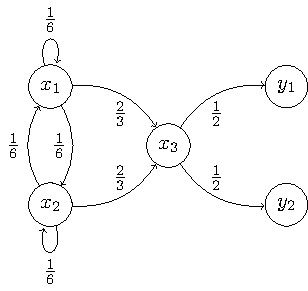
\includegraphics[width=\columnwidth]{./Figure/figure.pdf}
\caption { Markov Chain Diagram }
\end{figure}
\end {document}